\section{Исследовательская часть}

\subsection{Технические характеристики}

Технические характеристики устройства, на котором выполнялся замерный эксперимент:
\begin{itemize}[label*=---]
	\item операционная система Windows 11;
	\item память 16 ГБ;
	\item процессор 3,6 ГГц 6-ядерный процессор AMD Ryzen 5000 series 5.
\end{itemize}

Замеры проводились на ноутбуке, включенном в сеть электропитания. 
Во время тестирования ноутбук был нагружен только интегрированной средой разработки и непосредственно выполняемой программой.

\subsection{Пример работы программы}

На рисунке \ref{fig:example} представлен пример работы программы. 
Пользователь выбирает алгоритм умножения двух матриц из списка меню.
Вводит размеры матриц, их значения.
Программа вычисляет результат умножения и выводит его на экран.

\begin{figure}
	\centering
	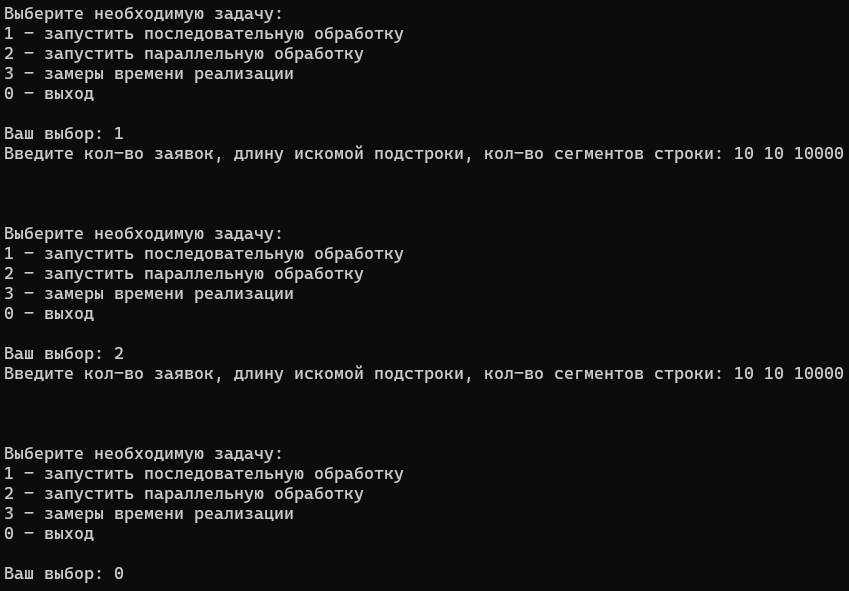
\includegraphics[width=0.4\linewidth]{images/example}
	\caption{Пример работы программы}
	\label{fig:example}
\end{figure}

\newpage

\subsection{Время выполнения реализованных алгоритмов}
Замеры времени работы реализованных алгоритмов для определенного размера квадратных матриц проводились 1000 раз, при этом каждый раз значения матриц генерировались случайно.

Для измерения тактового времени была использована инструкция rdtsc \cite{microsoft_rdtsc}.

В качестве результата, представленного на графике \ref{fig:timefull}, взято среднее время выполнения алгоритмов в тактах процессора для каждой матрицы размера от 1 до 10.

\begin{figure}
	\centering
	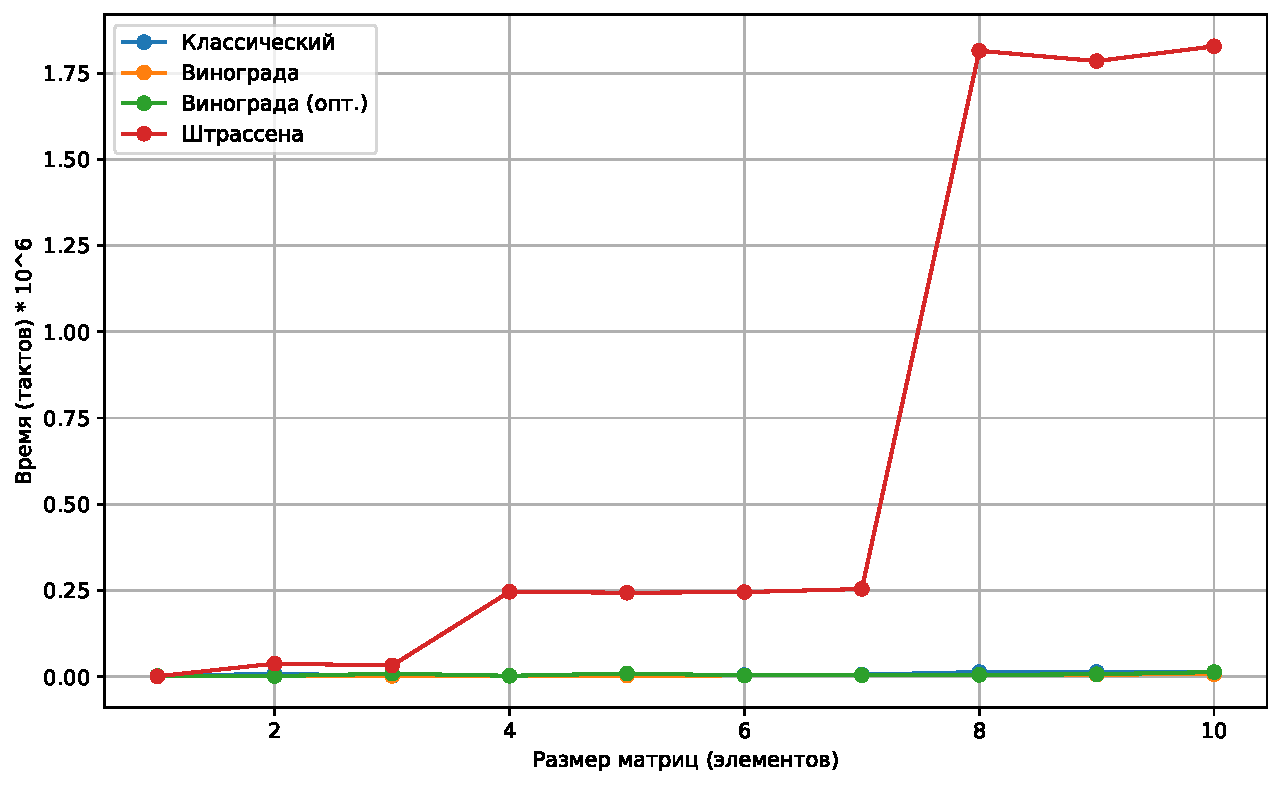
\includegraphics[width=0.9\linewidth]{../src/lab_02/timefull}
	\caption{Время выполнения алгоритмов}
	\label{fig:timefull}
\end{figure}

Тот же самый график, но без учёта алгоритма Штрассена:

\begin{figure}
	\centering
	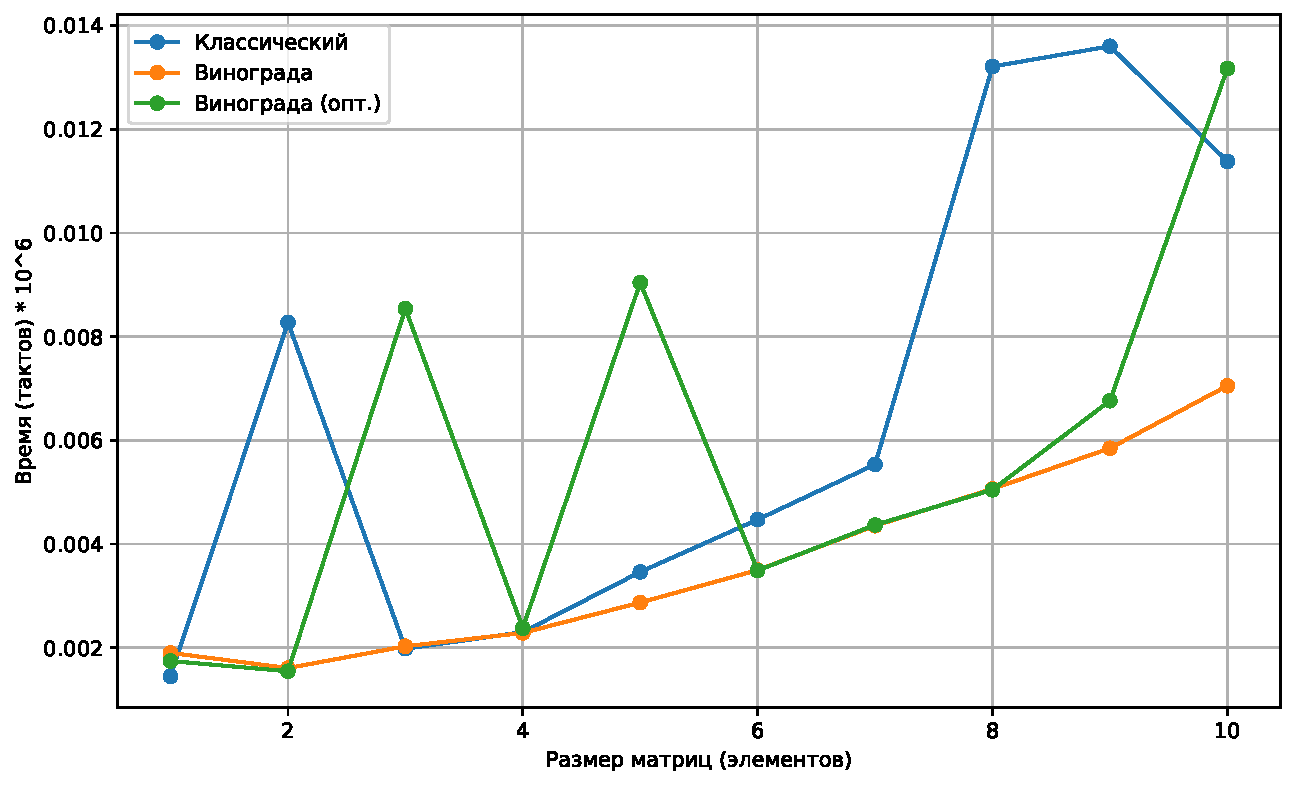
\includegraphics[width=0.9\linewidth]{../src/lab_02/time}
	\caption{Время выполнения алгоритмов (без учёта алгоритма Штрассена)}
	\label{fig:time}
\end{figure}

В половине случаев оптимизированная версия алгоритма Винограда работает дольше, чем \textit{обычный} алгоритм Винограда.

В результате трансляции кода программы на язык ассемблера, было замечено следующее: дизассемблированная строка исходного кода, выполняющая операцию вычисления значения \code{row[i]}, при оптимизированной реализации алгоритма Винограда содержит инструкции \code{lea} и \code{movsxd}, из-за чего количество выполняемых команд становится больше, чем в \textit{обычном} алгоритме Винограда.

Количество команд и, следовательно, разность в количестве инструкций также увеличивается при нечётном размере матриц.
Поэтому на графике заметны выбросы во времени у оптимизированного алгоритма Винограда.

Поэтому время выполнения увеличивается.

\newpage

\subsection{Занимаемая память реализованных алгоритмов}
 
График \ref{fig:memory} демонстрирует объём памяти в байтах, потребляемый разными реализациями алгоритмов в зависимости от размера матриц.
Занимаемый объём памяти считался как сумма размеров переменных, используемых в алгоритме и структуре данных.

\begin{figure}
	\centering
	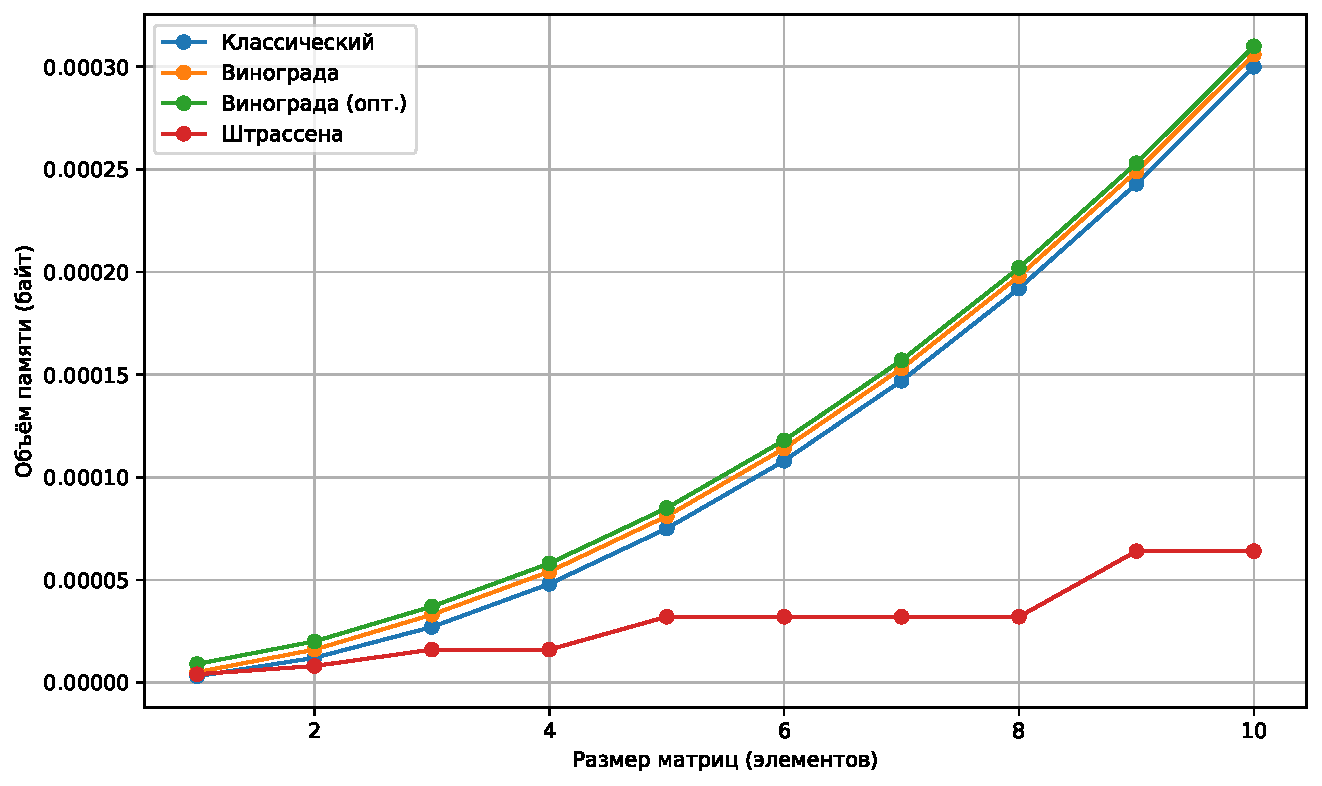
\includegraphics[width=0.9\linewidth]{../src/lab_02/memory}
	\caption{Объём памяти, используемый алгоритмами}
	\label{fig:memory}
\end{figure}


\subsection{Вывод}

В результате анализа замеров времени выполнения и затрат памяти на различных алгоритмах были сделаны следующие выводы:

\begin{itemize}
	\item алгоритм Штрассена занимает меньше всего памяти при размере квадратных матриц больше единицы;
	\item алгоритм Винограда и его оптимизированная версия быстрее всех умножают матрицы;
	\item разница во времени выполнения алгоритма Винограда и его оптимизированной версии зависит от процессора.
\end{itemize}